\subsection{Idealised model of a channel}

We now give an idealised model of a channel: this describes the behaviour of a
channel in terms of the calls and returns of functions, while abstracting away
from the implementation.  We assume (for simplicity) a single thread,
|AltThread|, that runs any alt that interacts with the channel.

%%%%% 

\begin{figure}
\begin{center}
\def\height{10mm} % height of boxes
\def\linW{15mm} % width of "Lin(t)" box
\def\gap{0.1} % gap for stacked figure
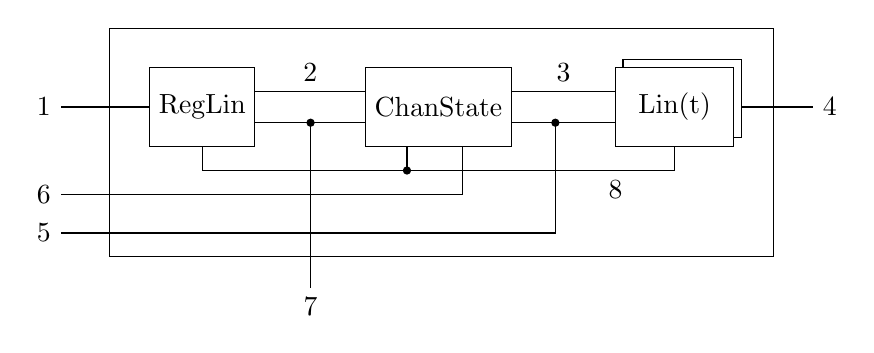
\begin{tikzpicture}
%%%%% RegLin
\draw (0,0) node[draw, minimum height = \height](regLin){\cspmstyle RegLin};
%% (1)
\draw (regLin) -- node[left, at end]{\inCircle{1}}  ++ (-1.8,0) 
  coordinate (left);
%%%%% ChanState
\draw (3,0) node[draw, minimum height = \height](chanState){
  \cspmstyle ChanState};
% syncs with RegLine
\path (regLin.east) -- ++(0,-0.2) coordinate (a) -- ++(0,0.4) coordinate(aa);
\path (chanState.west) -- ++(0,-0.2) coordinate (b) -- ++(0,0.4)
  coordinate(bb);
%% (2)
\draw (aa) -- node[above]{\inCircle{2}} (bb);
%% (7)
\draw (a) -- (b);  \fill (a) ++ (0.7,0) circle(1.5pt) coordinate (t1);
\draw (t1) -- node[below, at end]{\inCircle{7}} ++(0,-2.1);
%%%%% Lin
\draw (chanState) ++ (3,0) 
  node[draw, minimum height = \height, minimum width = \linW](lin){
    \cspmstyle Lin(t)};
\draw (lin.north west) ++ (\gap, 0.0) |- ++ (\linW, \gap) |- 
  ++ (-\gap, -\height);
%% (4)
\draw (lin.east) ++ (0.1,0) -- node[right, at end]{\inCircle{4}} 
  ++ (0.9,0) coordinate (right);
%% (6)
\path (chanState.south) -- ++ (0.3,0) coordinate (a);
\draw (a) -- ++ (0,-0.6) coordinate (temp) 
  -- node[left, at end]{\inCircle{6}} (temp -| left); 
% syncs between ChanState and Lin
\path (chanState.east) -- ++(0,-0.2) coordinate (a) -- ++(0,0.4) coordinate(aa);
\path (lin.west) -- ++(0,-0.2) coordinate (b) -- ++(0,0.4) coordinate(bb);
%% (3)
\draw (aa) -- node[above]{\inCircle{3}} (bb);
%% (5)
\draw (a) -- (b); \fill (a) ++ (0.55,0) circle(1.5pt) coordinate (t1);
\draw (t1) -- ++(0,-1.4) coordinate (temp) -- 
  node[left, at end]{\inCircle{5}} (temp -| left);
%%%%% Syncs between all three
%% (8)
\draw (regLin.south) -- ++ (0,-0.3) coordinate (a);
\path (chanState.south) -- ++ (-0.4,0) coordinate (c);
\draw (c) -- ++ (0,-0.3); \fill (c) ++ (0,-0.3) circle(1.5pt);
\draw (lin.south) -- ++ (0,-0.3) coordinate (b);
\draw (a) -- node[below, very near end]{\inCircle{8}} (b);
%%%%% Outer box
\path (regLin.west) -- ++ (-0.5,1) coordinate (a) -- ++(0,-2.9) coordinate (d);
\path (lin.east) --  ++(0.5,1) coordinate (b) -- ++(0,-2.9) coordinate (c);
\draw (a) -- (b) -- (c) -- (d) -- (a);
%
\end{tikzpicture}
\end{center}

%%%%%

\uncspMid
\textbf{Key.}  We use BNF-style notation to capture
channels with similar names; for example, we write
``\CSPM{(begin}\m\CSPM{end)Send}'' to denote the \CSPM{beginSend} and
\CSPM{endSend} channels.  The interface with an alt appears on the left; the
interface with channel-threads appears on the right; error events appear
below; internal events appear inside the box. 

\raggedright
%
\begin{itemize}
\item[\inCircle{1}:]  \CSPM{(begin}\m\CSPM{end)Register(In}\m\CSPM{Out)}, 
  \CSPM{(begin}\m\CSPM{end)Deregister(In}\m\CSPM{Out)};

\item[\inCircle{2}:] \CSPM{register(In}\m\CSPM{Out)Wait};
  \CSPM{deregister(In}\m\CSPM{Out)}, \CSPM{isClosed.AltThread};

\item[\inCircle{3}:] \CSPM{sync}, \CSPM{callMaybeSend},
  \CSPM{callMaybeReceive}, \CSPM{close}, \CSPM{isClosed}, \CSPM{commit},
  \CSPM{timeout};

\item[\inCircle{4}:] \CSPM{(begin}\m\CSPM{end)Send},
  \CSPM{(begin}\m\CSPM{end)Receive}, \CSPM{(begin}\m\CSPM{end)SendWithin},
  \CSPM{(begin}\m\CSPM{end)ReceiveWithin}, \CSPM{(begin}\m\CSPM{end)Close};

\item[\inCircle{5}:] \CSPM{(begin}\m\CSPM{end)MaybeReceive},
  \CSPM{(begin}\m\CSPM{end)MaybeSend};

\item[\inCircle{6}:] \CSPM{(begin}\m\CSPM{end)portClosed};

\item[\inCircle{7}:] \CSPM{registerError},
  \CSPM{deregister(In}\m\CSPM{Out)Error};

\item[\inCircle{8}:] \CSPM{register(In}\m\CSPM{Out)Sync}.
\end{itemize}
\caption{Construction of the idealised channel.  \label{fig:idealised-chan}}
\end{figure}

\cspMid

%%%%%

The construction is made more complicated by the fact that the model needs to
deal with the |begin| and |end| events for function calls, whereas these
functions will take effect at their linearisation points.  We therefore
construct the model from several components, as depicted in
Figure~\ref{fig:idealised-chan}.  The component |ChanState| keeps track of the
state of the channel: whether an alt is registered at a port, and whether the
channel is closed.  The component |RegLin| is responsible for linearising
registrations and deregistrations.  Each component |Lin(t)| is responsible for
linearising the function calls of channel-thread~|t|.  We describe these in
more detail below.  Some details of the definitions are unobvious, and were
found by trial and error: their correctness is evidenced by the subsequent
successful refinement checks. 

%%%%%

\begin{figure}
\begin{cspm}
RegLin = 
  beginRegisterIn.AltThread?alt?index -> RegLinRegIn(alt, index)
  [] beginDeregisterIn.AltThread?alt?index -> RegLinDeregIn(alt, index)
  [] beginRegisterOut.AltThread?alt?index -> RegLinRegOut(alt, index)
  [] beginDeregisterOut.AltThread?alt?index -> RegLinDeregOut(alt, index)
  
RegLinRegIn(alt, index) = 
  let endChan = endRegisterIn.AltThread.alt within
  registerInSync?t?x -> endChan.RegisterSuccess.x -> RegLin
  [] registerInWait.alt.index -> endChan.RegisterWaiting -> RegLin
  [] isClosed.AltThread -> endChan.RegisterClosed -> RegLin
  [] registerError -> STOP
  
RegLinDeregIn(alt, index) = 
  deregisterIn.alt.index -> endDeregisterIn.AltThread.alt -> RegLin
  [] deregisterInError.alt.index -> STOP
  
RegLinRegOut(alt, index) = 
  let endChan = endRegisterOut.AltThread.alt within
  (**|~| x : Data @ registerOutSync?t!x -> endChan.RegisterSuccess.x -> RegLin)
  [] registerOutWait.alt.index -> endChan.RegisterWaiting -> RegLin
  [] isClosed.AltThread -> endChan.RegisterClosed -> RegLin
  [] registerError -> STOP
  
RegLinDeregOut(alt, index) = 
  deregisterOut.a.index -> endDeregisterOut.AltThread.a -> RegLin
  [] deregisterOutError.a.index -> STOP
\end{cspm}
\caption{Definition of the {\cspmstyle RegLin} process, controlling
  registration and deregistration.  \label{fig:RegLin}}
\end{figure}

%%%%%

The |RegLin| process is defined in Figure~\ref{fig:RegLin}; it accepts the
relevant |begin| events, with each function being handled by a different
subprocess. 

The process |RegLinRegIn(alt, index)| models the linearisation of a
\SCALA{registerIn(alt, index)} call, which can happen in several ways.
%
\begin{itemize}
\item A synchronisation with a waiting \SCALA{send} by a channel thread~|t|,
  with the alt receiving~|x|, is modelled by an event~|registerInSync.t.x|;
  this synchronises with the corresponding |Lin(t)| process.

\item An unsuccessful registration is modelled by an
  event |registerInWait.alt.index|.

\item A registration that finds the channel closed is modelled by an event
  |isClosed.AltThread|.

\item In incorrect registration, where an alt is already registered, is
  modelled by the event |registerError|.
\end{itemize}
% 
The |ChanState| process synchronises on each of these events, to make sure the
correct one is selected, based on the current channel state. 

The process |RegLinRegOut(alt, index)| models the linearisation of a
\SCALA{registerOut(alt, index)} call, in a similar way.  The processes
|RegLinDeregIn(alt, index)| and |RegLinDeregOut(alt, index)| model
deregistrations, including the possibility of an erroneous deregistration.

%%%%%

\begin{figure}
\begin{cspm}
Lin(t) = 
  beginSend.t?x -> SendingLin(t, x, endSend.t, false)
  [] beginReceive.t -> ReceivingLin(t, endReceive.t, false)
  [] beginSendWithin.t?x -> SendingLin(t, x, endSendWithin.t, true)
  [] beginReceiveWithin.t -> ReceivingLin(t, endReceiveWithin.t, true) 
  [] beginClose.t -> close.t -> isClosed.t -> endClose.t -> Lin(t)
  
SendingLin(t, x, endChan, timed) = 
  let Success = endChan.SendSuccess -> Lin(t) within
  sync.t?t':ChanThread-{t}!x -> commit.t -> Success
  []
  registerInSync.t.x -> commit.t -> Success
  []
  callMaybeReceive.t?alt?index!x -> beginMaybeReceive.t.alt.index.x -> 
    endMaybeReceive.t.alt?res -> 
    (if res then Success else SendingLin(t, x, endChan, timed))
  []
  isClosed.t -> endChan.Closed -> Lin(t)
  []
  timed & timeout.t -> endChan.Timeout -> Lin(t)
  
ReceivingLin(t, endChan, timed) =  
  let Success(x) = endChan.ReceiveSuccess.x -> Lin(t) within
  sync?t':ChanThread-{t}!t?x -> Success(x) 
  []
  registerOutSync.t?x -> Success(x) 
  []
  callMaybeSend.t?alt?index -> beginMaybeSend.t.alt.index -> (
    endMaybeSend.t.alt.Some?x -> Success(x) 
    [] endMaybeSend.t.alt.None -> ReceivingLin(t, endChan, timed) )
  [] 
  isClosed.t -> endChan.Closed -> Lin(t)
  []
  timed & timeout.t -> endChan.Timeout -> Lin(t)
\end{cspm}
\caption{Definition of the {\scalashape Lin} processes, controlling
  channel-thread functions.  \label{fig:Lin}}
\end{figure}

%%%%%

The |Lin(t)| processes are defined in Figure~\ref{fig:Lin}.  Each accepts the
relevant \SCALA{begin} and \SCALA{end} events from channel-thread~|t|, with
most of the functions modelled by relevant subprocesses.

The process |SendingLin| models the linearisation of the \SCALA{send} and
\SCALA{sendWithin} functions; the parameter |timed| indicates the latter case.
The subprocess |Success| indicates a successful send.  There are several
cases.
%
\begin{itemize}
\item A synchronisation with another channel thread~|t'| is represented by the
  event |sync.t.t'.x|.  In the implementation, thread~|t| might not be able to
  return immediately: it must first obtain the lock.  This is modelled here by
  a synchronisation on event |commit.t| with |ChanState|, which might be
  blocked in some circumstances.

\item A synchronisation with an alt performing \SCALA{registerIn} is captured
  by the event |registerInSync.t.x|, described earlier.  Again, the thread~|t|
  might not be able to return immediately, as modelled here by a
  synchronisation on |commit.t|.

\item A decision to call |maybeReceive| on an alt~|alt| registered with
  index~|index| is modelled by the event |callMaybeReceive.t.alt.index.x|;
  this event is a synchronisation with |ChanState|, which allows it only when
  there is an alt registered at the inport, and sets the |alt| and |index|
  fields.  Thread~|t| then calls |maybeReceive|, waits to receive back the
  result, and reacts accordingly.

\item The thread can find the channel closed via the event |isClosed.t|.

\item In the case of the |sendWithin| function, the thread can timeout,
  modelled by the event |timeout.t|.  
\end{itemize}

The process |ReceivingLin| models the linearisation of the \SCALA{receive} and
\SCALA{receiveWithin}, in a similar way.  There is no need for the extra
synchronisation on the |commit| channel in this case: in the implementation,
these functions can return straightaway. 

Finally, the |Lin| processes directly deal with closing.  The event |close.t|
represents the linearisation point of the operation.  The \SCALA{close}
function might not be able to return immediately: the channel might need to
call \SCALA{portClosed} on a registered port (modelled within |ChanState|),
and wait for that call to return; the event |isClosed.t| becomes available at
that point.

%%%%%
 
\begin{figure}
\begin{cspm}
ChanState(regStatus) = 
  let regIns = getRegIns(regStatus)
      regOuts = getRegOuts(regStatus)
  within
  regStatus == NoReg & (
    registerInSync?t.x -> ChanState(NoReg) 
    [] registerOutSync?t.x -> ChanState(NoReg)
    [] registerInWait?alt?index -> ChanState(InReg.alt.index)
    [] registerOutWait?alt?index -> ChanState(OutReg.alt.index)
    [] deregisterIn?alt?index ->  ChanState(NoReg)
    [] deregisterOut?alt?index ->  ChanState(NoReg)
  )
  []
  regStatus != NoReg & (
    registerError -> STOP
    [] deregisterIn?(alt.index):regIns ->  ChanState(NoReg)
    [] deregisterOut?(alt.index):regOuts -> ChanState(NoReg)
    [] deregisterInError?(alt.index):AltIndex-regIns -> STOP
    [] deregisterOutError?(alt.index):AltIndex-regOuts -> STOP
    [] callMaybeReceive?t?(alt.index):regIns?x -> beginMaybeReceive.t.alt.index.x -> 
         endMaybeReceive.t.alt?res -> ChanState(NoReg)
    [] callMaybeSend?t?(alt.index):regOuts -> beginMaybeSend.t.alt.index -> 
         endMaybeSend.t.alt?res -> ChanState(NoReg)
  )
  [] 
  sync?t1?t2:others(t1)?x -> ChanState(regStatus)
  []
  commit?t -> ChanState(regStatus)
  []
  timeout?t -> ChanState(regStatus)
  []
  close?t -> (
    if regStatus == NoReg then ChanStateClosed
    else    
      beginPortClosed.t?(alt.index):regIns£$\union$£regOuts ->
      endPortClosed.t.alt -> ChanStateClosed
  )
\end{cspm}
\caption{The {\scalashape ChanState} process.  \label{fig:ChanState}}
\end{figure}

%%%%%

The |ChanState| process is in Figure~\ref{fig:ChanState}.  The parameter
|regStatus| records the current registration status, and is taken from the
following type.
%
\begin{cspm}
datatype RegStatus = NoReg | InReg.AltID.Index | OutReg.AltID.Index
\end{cspm}
%
where |AltID| is the type of alt identities, and |Index| is the type of
indices of branches.  The subtypes of |RegStatus| represent that no alt is
currently registered, or that an alt is registered at the inport or outport
corresponding to a particular index.  

In the definition of |ChanState|, the values |regIns| and |regOuts| store the
(empty or singleton) sets of |AltID.Index| pairs corresponding to
registrations at the inport or outport, respectively (these are calculated
using straightforward helper functions).

Several possibilities are available when there is no registered alt.
%
\begin{itemize}
\item A \SCALA{registerIn} or \SCALA{registerOut} operation may synchronise
  with a waiting channel thread.

\item A \SCALA{registerIn} or \SCALA{registerOut} operation may fail to
  synchronise; the registration status is updated appropriately.

\item A \SCALA{deregisterIn} or \SCALA{deregisterOut} operation may happen;
  which has no effect.  These events can arise if an alt is trying to
  deregister concurrently with an unsuccessful call back of
  \SCALA{maybeReceive} or \SCALA{maybeSend}, which clears the registration
  status. 
\end{itemize}

Several possibilities are available when there is a registered alt.
%
\begin{itemize}
\item Another registration attempt would be erroneous, represented by the
  event |registerError|.

\item The currently registered alt might be deregistered.

\item An attempt to deregister a different alt would be erroneous (here
  |AltIndex| represents the set of all |AltID.Index| pairs).

\item A channel thread~|t| may decide to call \SCALA{maybeReceive} or
  \SCALA{maybeSend} corresponding to the current registration.  The call is
  made and returns, and the registration is cleared (regardless of the
  result). 
\end{itemize}
%
Note that other events are blocked during calls to \SCALA{maybeReceive} or
\SCALA{maybeSend}; this corresponds to the fact that in the implementation,
the relevant channel-thread keeps the lock on the channel.

Other possibilities are available regardless of the registration status.
%
\begin{itemize}
\item Two threads~|t1| and |t2| may synchronise on a communication.

\item A sending thread~|t| may commit to returning (see the earlier
  explanation concerning the |Lin(t)| process). 

\item A channel-thread in a \SCALA{sendWithin} or \SCALA{receiveWithin} can
  timeout. 

\item The channel can be closed.  If there is a registered port, the channel
  calls |portClosed| on the relevant alt, and waits for it to return.
\end{itemize}

%%%%%

\begin{figure}
\begin{cspm}
ChanStateClosed = 
  isClosed?t -> ChanStateClosed
  [] close?t -> ChanStateClosed
  [] commit?t -> ChanStateClosed
  [] deregisterIn?alt?index -> ChanStateClosed
  [] deregisterOut?alt?index -> ChanStateClosed
\end{cspm}
\caption{The {\scalashape ChanStateClosed}
  process.  \label{fig:ChanStateClosed}}
\end{figure}

%%%%%

The process~|ChanStateClosed| in Figure~\ref{fig:ChanStateClosed} corresponds
to the channel having been closed.  
%
\begin{itemize}
\item This process can perform |inClosed.t|, synchronising with either
  |RegLin| (if |t| is the alt-thread) or |Lin(t)|, as described earlier.

\item The channel could be closed again (having no effect).

\item The process could synchronise with a |Lin(t)| process on event
  |commit.t|: this corresponds to sending thread~|t| having synchronised with
  another thread before the channel was closed. 

\item A deregistration may happen, which has no effect: this corresponds to
  the alt-thread starting the deregistration concurrently with the callback of
  |portClosed|. 
\end{itemize}

The components are combined together as illustrated in
Figure~\ref{fig:idealised-chan}, hiding all the internal events (those inside
the box in the figure).  This produces a process |ChannelSpec|.  Recall that
we want to allow arbitrary behaviour after one of the events that represents
that the environment has not followed the alt protocol, on channels
|registerError|, |deregisterInError| and |deregisterOutError|.  In the
stable-failures model, the process |CHAOS(Interface)| allows arbitrary
behaviour over the set |Interface| (the interface of the channel); in the
failures-divergences model, the process |DIV| allows arbitrary behaviour.  We
therefore define the following. 
%
\begin{cspm}
Errors = {|registerError, deregisterInError, deregisterOutError|}
Spec£$_F$£ = (ChannelSpec [|Errors|> CHAOS(Interface) ) \ Errors
Spec£$_D$£ = (ChannelSpec [|Errors|> DIV ) \ Errors
\end{cspm}

We can then compare the CSP model of a synchronous channel implementation
against the idealised model.  We create a system using the model of the
implementation, allowing threads to call appropriate operations.  We can then
verify that this system refines |Spec|$_F$ and |Spec|$_D$ in the relevant
models. 

\framebox{**} Number of threads, timing.  FD check faster than F check. 

 
